\chapter{Propuesta Blockchain basada en tiempo confiable}

XXXXXXXXXXXXXXXXXXXXXXXXXXXXXXXXXXXXXXXXXXXXX\newline

En base al protocolo actual que se tiene para las redes blockchain basadas en prueba de trabajo, ninguna de estas puede ser un sistema escalable. Si se quiere que una red blockchain basada en prueba de trabajo siga teniendo las características necesarias para sustentar una moneda digital, no se podrá conseguir que el sistema sea escalable como tal. Está diseñado para que sea ineficiente. Sin embargo, es posible hacer cambios en el protocolo para que, dentro de esa ineficiencia, el sistema sea lo más eficiente posible. \newline

¿Por qué está diseñado para ser ineficiente? La prueba de trabajo plantea problemas matemáticos a toda la red de usuarios de manera que el primero en encontrar la solución, la distribuya, sea el creador del siguiente bloque de la cadena y se lleve una recompensa por ello. El problema está en la distribución de la solución. Se necesita que la mayoría de la red esté de acuerdo con que un usuario en concreto ha sido el primero en encontrar la solución a la prueba de trabajo y todo lo que ello acarrea. El consenso debe llegar antes de que los usuarios de la red comiencen a buscar solución a la nueva prueba de trabajo. Los usuarios forman una red P2P, por lo que la distribución de la solución llevará su tiempo antes de que la mayoría de la red alcance el consenso. Para este tiempo es para el que se ajusta la dificultad de la prueba de trabajo, y no se puede reducir ya que sino la red no alcanzaría el consenso. En la red Bitcoin este tiempo es de aproximadamente 10 minutos. Suele ocurrir que, durante este tiempo de difusión de una solución, haya otros usuarios que, sin saber que alguien ya ha encontrado una solución, encuentren otra solución al mismo problema y comiencen a distribuirla desde otro punto de la red. Habrá usuarios de la red que reciban soluciones a la misma prueba de trabajo de distintos usuarios. Sólo una de ellas se puede considerar válida, y los usuarios deben ponerse de acuerdo en cuál de ellas. Cada vez que se encuentra una solución a la prueba de trabajo, a su vez se genera una nueva prueba de trabajo relacionada con esa solución anterior. El protocolo actual dicta que cuando un usuario recibe varias soluciones válidas a una misma prueba de trabajo, este debe elegir una de estas soluciones al azar y comenzar a buscar solución a la nueva prueba de trabajo generada. Cada usuario espera que la mayoría de la red haya elegido la misma solución que él, ya que sino estará buscando solución a una nueva prueba de trabajo distinta a la de la mayoría de la red y por ende inválida. Cuantas más soluciones se encuentren a la misma prueba de trabajo, más difícil resultará alcanzar el consenso. Por lo tanto, la dificultad de la prueba de trabajo se ajustará para que el número de soluciones concurrentes sea el mínimo posible.
A priori se puede pensar que resultaría mucho más eficiente que cada usuario sellara temporalmente su solución. Así cuando otro usuario de la red tenga que elegir entre varias soluciones, podrá hacerlo en base al sello temporal y no por azar. Esto da pie a otro de los puntos clave de las redes blockchain, y es que, al tratarse de redes P2P públicas, ningún usuario debe confiar en ningún otro. Por lo tanto, hay dos aspectos de los que ningún usuario debe fiarse:
\begin{enumerate}
	\item No se tiene la certeza de que otro usuario selle temporalmente una solución con la hora real de su reloj. Podría hacerlo con una hora previa para sacar ventaja de ello.
	\item No se tiene la certeza de que la hora real que marque el reloj de un usuario esté sincronizada con la hora UTC.
\end{enumerate}

El objetivo del presente trabajo consiste en solventar estos dos puntos. De conseguirlo, se podría hacer uso de un sellado temporal distribuido y confiable para las distintas soluciones que se encuentren a la prueba de trabajo. Se considera que esto permitiría a los usuarios de la red encontrar el consenso de manera más eficiente. Así se podría reducir la dificultad de la prueba de trabajo, sin que esto afecte al consenso, lo que supondría una mejora en el número de transacciones por segundo.\newline

XXXXXXXXXXXXXXXXXXXXXXXXXXXXXXXXXXXXXXXXXXXXXX


En el apartado de ObjetivosXXXXXXXXXXXXXXX se describen los principales problemas que tienen las redes blockchain públicas basadas en prueba de trabajo. El presente trabajo tiene como objetivo atajar el problema de la escalabilidad, no para hacer de estas redes blockchain un sistema escalable como tal, sino para intentar sacar el mayor rendimiento posible. El principal factor limitante para la escalabilidad nace de la prueba de trabajo. Sin embargo, ya se ha visto por qué la prueba de trabajo no se puede facilitar si se quiere que la red mantenga el consenso. La propuesta de este trabajo consiste en un sistema que permita hacer la prueba de trabajo más fácil manteniendo el consenso de la red. Para esto es necesario ahondar más en las consecuencias para comprender la propuesta.

\section{Forks en blockchain}
Para entender completamente en qué consiste un fork y las consecuencias que estos pueden acarrear en las cadenas de bloques se hace uso de un paper que estudia la propagación de los bloques por la red Bitcoin \cite{forks}. \newline

\begin{figure}
	\centering
	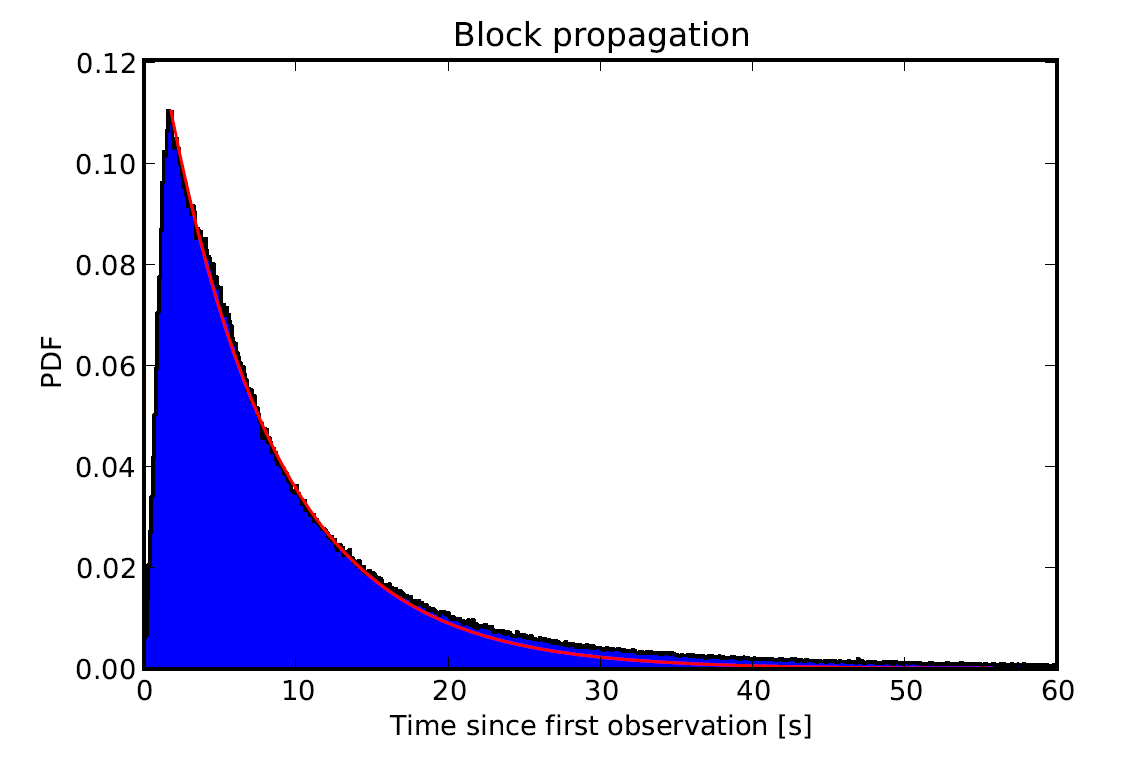
\includegraphics[width=1\textwidth]{imagenes/figura1.PNG}
	\caption{\label{fig1}Tiempo de propagación de un bloque \cite{forks}.}
\end{figure}

En el estudio se analiza en un primer momento el retardo de la red blockchain de Bitcoin. Se denomina retardo D al tiempo que tarda un bloque emitido por un minero en llegar al resto de la red. En la figura XXXXXXXXXXX se observa el resultado obtenido tras analizar 10000 bloques de la cadena. El retardo medio es de 12.6 segundos. Pasados 40 segundos aún hay un 5\% de los nodos que no han recibido el bloque. El objetivo de medir este retardo es ver su interacción real con el número de forks que se suceden en la red. Cuando el primer minero de la red consigue minar el bloque de altura (o longitud) N+1, inmediatamente lo emite a la red. Desde esta emisión transcurre un tiempo hasta que el resto de mineros de la red recibe este bloque. Durante este tiempo denominado D, el resto de los nodos de la red siguen intentando minar el bloque N+1 ya que aún no se han enterado de que otro minero ya ha conseguido minarlo. Si dentro de este tiempo D algún otro minero consigue minar otro bloque N+1, se tendrán 2 bloques N+1 emitidos a la red. Estos dos bloques se denominan (N+1) y (N+1)’. En este momento se podría dar el caso de que una parte de la red tome como válida la cadena que acaba con el bloque (N+1) y otra parte tome la cadena que acaba con el bloque (N+1)’. Habría que esperar al minado de varios bloques más para que la red se ponga de acuerdo en una única cadena, suponiendo esto un desperdicio de poder computacional y tener que revertir una cadena de longitud considerable (PUEDE QUE NO SE ENTIENDA LO DE REVERTIR CADENA QUITARLO???XXXXXXXXXXXXX). Cuanto mayor sea el tiempo D mayor es la probabilidad de que se produzcan forks en la red. \newline

\begin{figure}
	\centering
	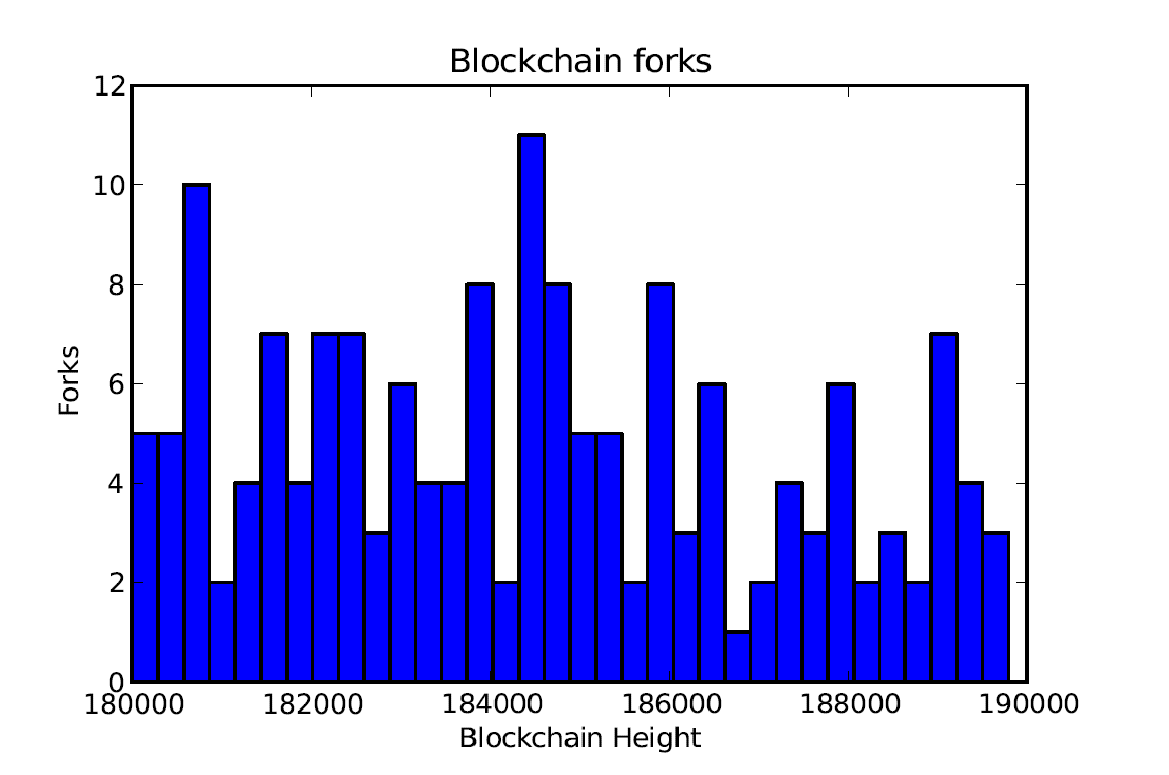
\includegraphics[width=1\textwidth]{imagenes/figura2.PNG}
	\caption{\label{fig1}Nº de forks con nodo en modo pasivo \cite{forks}.}
\end{figure}

El estudio pasa a medir el número de forks que se observan en un intervalo de 10000 bloques. Para ello monta un nodo “pasivo” que está conectado a una gran cantidad de nodos (bastante más grande de lo normal) con el objetivo de observar la mayor parte de la red posible. En la figura XXXXXXXXXX se observa que se producen un total de 169 forks en los 10000 bloques (r=1.69\%). En un intento por demostrar la repercusión del tiempo D en los forks producidos en la red, realizan un experimento en el que aumentan la conectividad de la red. Para ello hacen uso del anterior nodo con gran cantidad de nodos conectados, pero en modo “activo” (en este caso actuará en base al protocolo haciendo broadcast de la cadena más larga que conozca en cada momento). De nuevo miden durante 10000 bloques el número de forks, los resultados se observan en la figura XXXXXXXXXXXXXx. La tasa de forks pasa de un 1.69\% a un 0.78\%, esto supone una mejora de un 53.41\% en el número de forks. La conclusión que se obtiene de este estudio es que aumentar la conectividad de un nodo (400 conexiones frente a las 8 que suele tener un nodo) ha provocado un descenso considerable en la tasa de forks. Esto se ha producido por el simple hecho de que se ha conseguido alcanzar el consenso en una misma cadena más rápido que si se tuviese que esperar a que alguna cadena adelante a otra (en número de bloques). Si un nodo ha recibido 2 cadenas bien formadas distintas de la misma longitud, tendrá que elegir una al azar. Si muchos nodos eligen con qué cadena quedarse al azar el resultado será que no haya consenso hasta más adelante. Este es el principal foco de atención de este trabajo, conseguir que ningún nodo tenga que elegir al azar con qué cadena quedarse en ningún momento. \newline


\begin{figure}
	\centering
	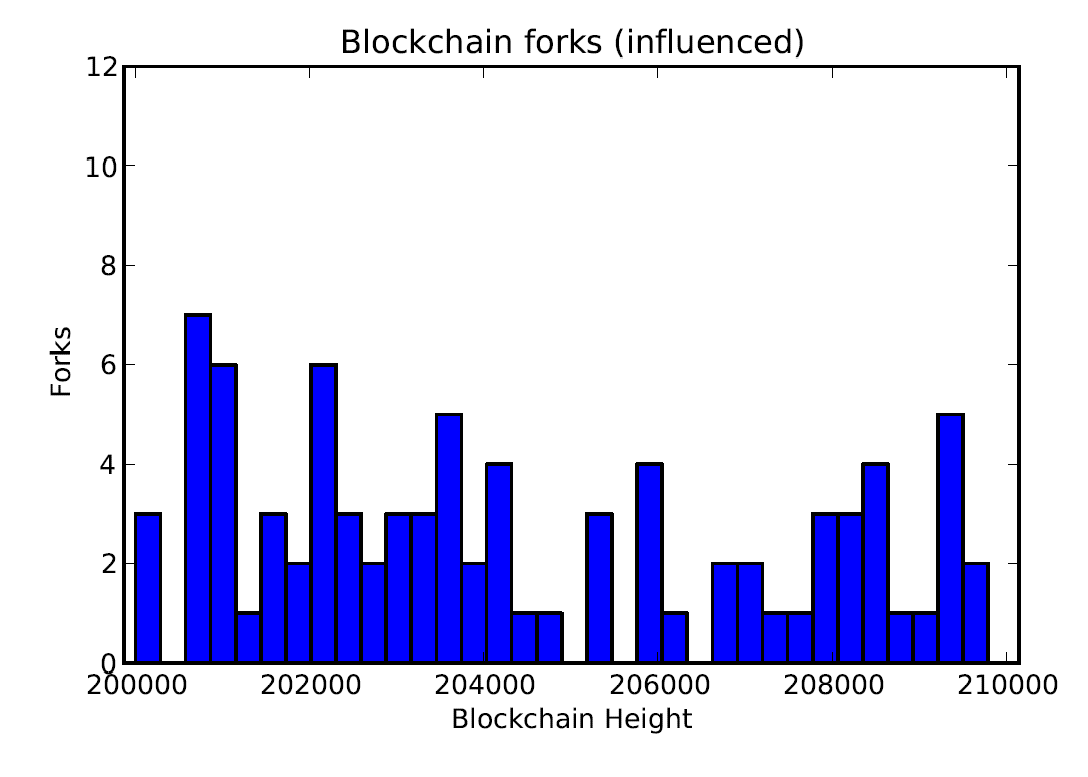
\includegraphics[width=1\textwidth]{imagenes/figura3.PNG}
	\caption{\label{fig1}Nº de forks con nodo en modo activo \cite{forks}.}
\end{figure}

El número de forks no solamente es un problema para el consenso, sino también para la seguridad. Para ver por qué, se hace uso de un artículo hecho para la red Bitcoin \cite{ghost} que explica por qué una disminución del tiempo de la prueba de trabajo (que aumente la tasa de transacciones por segundo), que se traduciría en un incremento de los forks, haría la blockchain más vulnerable. 

\begin{figure}
	\centering
	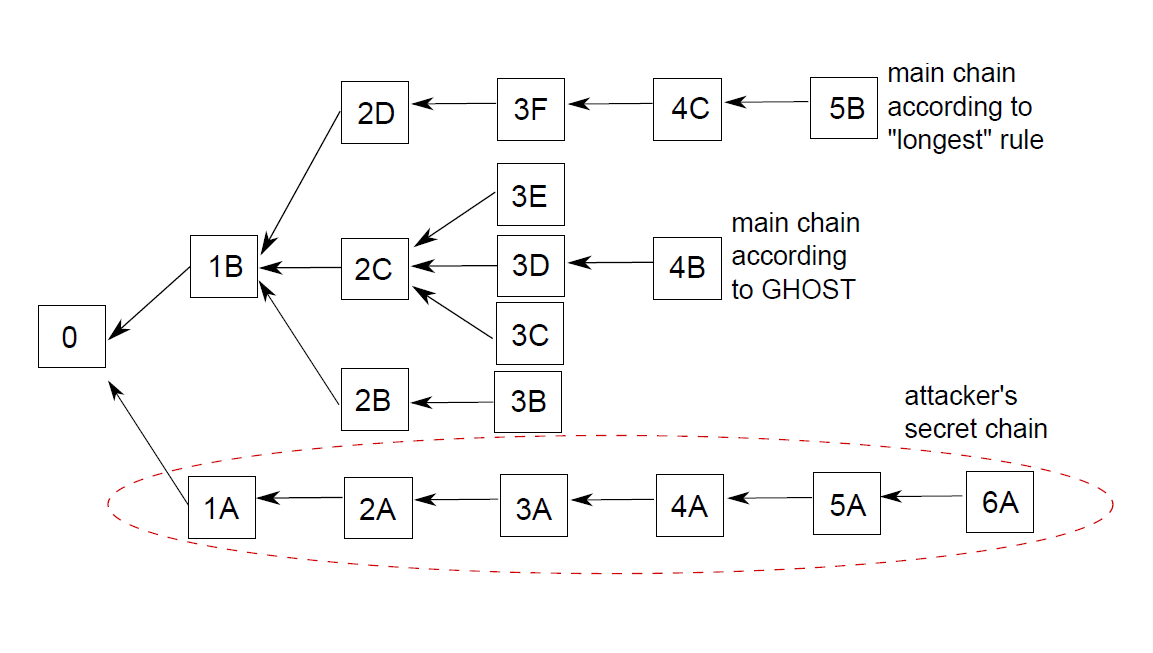
\includegraphics[width=1\textwidth]{imagenes/figura5.PNG}
	\caption{\label{fig1}Estrategia "Self-Mine-Strategy" \cite{ghost}.}
\end{figure}

La figura XXXXXXXXXXx muestra una situación en la que un atacante intenta realizar un ataque del 51\%. Se supone que el atacante tiene un poder computacional del 30\% y el resto de la red honesta dispone del 70\% restante. Disminuir el tiempo de la prueba de trabajo conlleva un mayor número de forks. Cuando se producen varios forks, la parte honesta de la red está divida en tantas partes como forks haya. A la altura del bloque número 2 de la figura XXXXXXXxxxx se tienen 3 forks, por tanto, el 70\% del poder computacional de la red honesta estará dividido en estos 3 forks. Cada parte de la red estará intentando minar el siguiente bloque de la cadena sobre una de las 3 cadenas distintas que se tiene. El atacante está actuando por su cuenta, así que emplea el 30\% de su poder computacional íntegramente en minar sobre su única cadena. A esta técnica de minado del atacante se la denomina “Self-Mine-Strategy”. Es evidente que el atacante con sólo el 30\% del poder computacional de la red será capaz de crear una cadena más larga que el resto de la red honesta y llevará su ataque con éxito. \newline

Esta situación se podría haber evitado con la propuesta que presenta este trabajo. Si se observa con detenimiento la figura XXXXXXXXXXXXX, se ve que los forks que se han producido a la altura de los bloques 2 y 3 se debe a que los nodos han recibido varias cadenas de igual longitud y han tenido que elegir una de ellas al azar. Si se consigue evitar esta situación en la que los nodos no sepan qué cadena de igual longitud (en número de bloques) elegir, se mantendría el consenso en una misma cadena. Manteniendo el consenso en una sola cadena haría que toda la parte honesta de la red volcase todo su poder computacional (70\%) en la misma cadena y el atacante con su 30\% no pueda llevar a cabo el ataque. \newline

La situación idílica en el caso de que se produzca un fork sería no sólo que todos los nodos que están en esta situación elijan la misma cadena, sino que todos elijan la primera que realmente se minó. A priori se podría pensar que, si el minero añadiese un timestamp al bloque al minarlo, el resto podría saber fácilmente qué cadena se minó la primera. El timestamp en blockchain es un tema algo controvertido que merece la pena tratar, sobre todo para la propuesta del trabajo.\newline

\section{El papel del timestamp en blockchain}
Una situación que a menudo es confusa de blockchain es la puntual falta de orden temporal del timestamp de los bloques. En repetidas ocasiones un bloque posee un timestamp menor al timestamp de un bloque previo. En base a la mayoría de los protocolos blockchain actuales, esta situación es totalmente válida. \newline

Una red blockchain no posee una autoridad central que informe del tiempo UTC (Universal Time Coordinated). Asumir que el tiempo local de cada nodo es preciso o está sincronizado con los relojes del resto es un error. Cada nodo está conectado a la red a través de una serie de pares. Cada nodo posee un tiempo UTC local con un offset marcado por la media del tiempo UTC local de cada par (peer?????XXXX) a los que está conectado. El tiempo global de la red blockchain está marcado por la media de los timestamps emitidos por todos y cada uno de los nodos de la red. Esto provoca que la sincronización en estas redes no sea nada óptima, provocando situaciones en las que el orden de los timestamps no sea correcto. \newline

El protocolo de Bitcoin únicamente rechaza un timestamp si es menor a la media de los timestamps de los 11 bloques anteriores o 2 horas superior al tiempo global de la red. De manera parecida se realiza en Ethereum, provocando que un nodo pueda falsear su timestamp en unos 900 segundos sin repercusión alguna.

